\documentclass{beamer}
\usepackage{geometry}
\usepackage[english]{babel}
\usepackage[utf8]{inputenc}
\usepackage{amsmath}
\usepackage{amsfonts}
\usepackage{amssymb}
\usepackage{tikz}
\usetikzlibrary{quotes, angles}
\usepackage{graphicx}
\usepackage{multicol}

%\usepackage{pgfplots}
%\pgfplotsset{width=10cm,compat=1.9}
%\usepackage{pgfplotstable}

\setlength{\headheight}{26pt}%doesn't seem to fix warning

\usepackage{fancyhdr}
\pagestyle{fancy}
\fancyhf{}

%\rhead{\small{3 September 2019}}
\lhead{\small{BECA / Dr. Huson / Geometry Unit 1}}

\renewcommand{\headrulewidth}{0pt}

\title{Mathematics Class Slides}
\subtitle{Bronx Early College Academy}
\author{Christopher J. Huson PhD}
\date{21-25 September 2020}

\begin{document}
\frame{\titlepage}
\section[Outline]{}
\frame{\tableofcontents}

\section{1.1 1st day of Geometry, Segment addition, 21 Sept}
\frame
{
  \frametitle{GQ: How do we define the basic elements of geometry?}
  \framesubtitle{CCSS: HSG.CO.A.1 Know precise geometric definitions \hfill \alert{1.1 Monday 21-22 Sept}}

  Welcome back to school
  \begin{block}{Do Now: Algebra skills check}
  \begin{enumerate}
      \item Remote learning attendance
      \item Take out notebooks (or blank paper)
      \item Complete Do Now on Google Classroom
  \end{enumerate}
  \end{block}
  Supply list: Composition book, folder, looseleaf, pencils \& pens, \\*
  compass and ruler, calculator \\
  Lesson: Points, line segments, length; Segment addition postulate \\
  Homework: Begin Khan Academy unit (due Friday)
}

  \frame
  {
    \frametitle{Take class notes in a composition book}
    \begin{block}{Use this notebook format (required)}
      \begin{enumerate}
        \item In the front, write your name, my contact info, your passwords
        \item Each page in the top left corner: \\ \qquad First+Last Name \\
        \qquad 21 September 2020 \\ \qquad 1.1 Segment addition postulate \vspace{0.25cm}
        \item Copy definitions using your own words
        \item Write down example diagrams and problems
      \end{enumerate}
      \end{block}
    Point: a location, a dot, has no size; label with capital letter, $P$ \\[0.25cm]
    Line segment: two points and all the points between them; label with \emph{end points} and a bar, $\overline{AB}$ \\
  }

  \frame
  {
    \frametitle{Example: Points and line segments}
    Shown points $P$, $A$, $B$, $C$, line segments $\overline{AB}$, $\overline{BC}$\\[0.15in]
       \begin{tikzpicture}
        \draw [fill] (1,2) circle [radius=0.05] node[below]{$P$};
        \draw [-, thick] (0,1)--(3,1);
        \draw [fill] (0,1) circle [radius=0.05] node[below]{$A$};
        \draw [fill] (3,1) circle [radius=0.05] node[below]{$B$};
        \draw [-, thick] (3,0)--(7,0);
        \draw [fill] (3,0) circle [radius=0.05] node[below]{$B$};
        \draw [fill] (7,0) circle [radius=0.05] node[below]{$C$};
      \end{tikzpicture} \\ \vspace{0.5cm}
      Given $AB=3$, $BC=4$.\\[0.5cm]
      Notation: the length of a line segment is written as the two end points without a bar over them, $AB$.
  }

  \frame
  {
    \frametitle{Example: Points and line segments}
    \framesubtitle{Segment Addition Postulate}
    Shown \emph{collinear} points $A$, $B$, $C$. Given $AB=3$, $BC=4$. \\[0.15in]
    Find $AC$. \\[0.25in]
       \begin{tikzpicture}
        \draw [fill] (0,0) circle [radius=0.05] node[below]{$A$};
        \draw [-, thick] (0,0)--(7,0);
        \draw [fill] (3,0) circle [radius=0.05] node[below]{$B$};
        \draw [fill] (7,0) circle [radius=0.05] node[below]{$C$};
        \node at (1.5,0) [above]{$3$};
        \node at (5,0) [above]{$4$};
        \draw [<->, dashed] (0,-1)--(7,-1);
        \node at (3.5,-1) [below]{$?$};
      \end{tikzpicture} \\ \vspace{1cm}
      
      Definition: Points are \emph{collinear} when they lie on a straight line.
  }

  \frame
  {
    \frametitle{Example 2: Points and line segments}
    \framesubtitle{Segment Addition Postulate}
    Given collinear points $Q$, $R$, $S$, with $QR=11$, $QS=20$. \\[0.15in]
    Find $RS$. \\[0.25in]
       \begin{tikzpicture}
        \draw [fill] (0,0) circle [radius=0.05] node[below]{$Q$};
        \draw [-, thick] (0,0)--(7,0);
        \draw [fill] (3.8,0) circle [radius=0.05] node[below]{$R$};
        \draw [fill] (7,0) circle [radius=0.05] node[below]{$S$};
        \node at (1.7,0) [above]{$11$};
        \node at (5.2,0) [above]{$x$};
        \draw [<->, dashed] (0,-1)--(7,-1);
        \node at (3.5,-1) [below]{$20$};
      \end{tikzpicture} \\ \vspace{0.2cm}
      \begin{enumerate}
        \item How would you check your answer?
        \item Which equation represents the situation?
        \begin{multicols}{2}
          $11 + x = 20$ \\
          $x = 20 - 11$
        \end{multicols}
      \end{enumerate}
  }

  \frame
  {
    \frametitle{Example 3: Segment addition postulate}
    
    Given $\overline{JKL}$, $JK=2x+3$, $KL=5$, $JL=12$. Find ${x}$.\\[0.15in]
       \begin{tikzpicture}
        \draw [-, thick] (0,0)--(7,0);
        \draw [fill] (0,0) circle [radius=0.05] node[below]{$J$};
        \draw [fill] (4,0) circle [radius=0.05] node[below]{$K$};
        \draw [fill] (7,0) circle [radius=0.05] node[below]{$L$};
        \node at (1.7,0) [above]{$2x+3$};
        \node at (5.5,0) [above]{$5$};
        \draw [<->, dashed] (0,-1)--(7,-1);
        \node at (3.5,-1) [below]{$12$};
      \end{tikzpicture} %\vspace{1cm}
  \begin{enumerate}
      \item Write down an equation to represent the situation. \vspace{1cm}
      \item Solve for $x$. \vspace{1cm}
      \item Check your answer.
    \end{enumerate}
  }

  \frame
  {
    \frametitle{Example 4 (challenge): Segment addition postulate}
    
    Given $\overline{ABC}$, $AB=3x-7$, $BC=x+5$, $AC=14$. Find ${AB}$.\\[0.5in]
       \begin{tikzpicture}
        \draw [-, thick] (0,0)--(7,0);
        \draw [fill] (0,0) circle [radius=0.05] node[below]{$A$};
        \draw [fill] (3,0) circle [radius=0.05] node[below]{$B$};
        \draw [fill] (7,0) circle [radius=0.05] node[below]{$C$};
      \end{tikzpicture} \vspace{1cm}
  }

  \section{1.2 Segment addition, midpoint, 23 Sept}
  \frame
  {
    \frametitle{GQ: How do we solve for segment lengths?}
    \framesubtitle{CCSS: HSG.CO.A.1 Know precise geometric definitions  \hfill \alert{1.2 Wedn 23-24 Sept}}
  
    \begin{block}{Do Now: Complete Google Form in G-Classroom}
    %\begin{enumerate}
        %\item
    %\end{enumerate}
    \end{block}
    Lesson: \\ Point, line segment, end point, collinear, distance or length; \\ line, ray, plane, coplanar, congruent, angle, vertex \\*[5pt]
    Midpoints, bisectors, practice segment addition situations
  }

  \frame
  {
    \frametitle{Review: points, segments, length}
    Give an example of each geometric object. Use proper notation.
    \begin{enumerate}
      \item point
      \item line segment
      \item end point
      \item three collinear points
       \begin{tikzpicture}
        \draw [fill] (6,2) circle [radius=0.05] node[below]{$Q$};
        \draw [-, thick] (0,2)--(3,1);
        \draw [fill] (0,2) circle [radius=0.05] node[below]{$R$};
        \draw [fill] (3,1) circle [radius=0.05] node[below]{$S$};
        \draw [-, thick] (4,0)--(7,3);
        \draw [fill] (4,0) circle [radius=0.05] node[above left]{$T$};
        \draw [fill] (7,3) circle [radius=0.05] node[below right]{$U$};
      \end{tikzpicture}
      \item Given $TQ=1.4$, $QU=0.6$. Find $TU$.
    \end{enumerate}
  }

  \frame
  {
    \frametitle{More definitions: lines, rays, planes}
    A \emph{line} extends infinitely in both directions, $\overleftrightarrow{AB}$. \\
    (sometimes labeled with a small letter, for example, line $k$) \\[0.15in]
    \begin{center}
      \begin{tikzpicture}
        \draw [<->, thick] (0,1)--(5,1);
        \node at (0.25, 1)[above]{$k$};
        \draw [fill] (1.5,1) circle [radius=0.05] node[below]{$A$};
        \draw [fill] (3.5,1) circle [radius=0.05] node[below]{$B$};
      \end{tikzpicture}
    \end{center}
      A \emph{ray} has one end point and extends infinitely in one direction, $\overrightarrow{CD}$. \\[0.15in]
      \begin{center}
          \begin{tikzpicture}
        \draw [->, thick] (3,0)--(7,0);
        \draw [fill] (3,0) circle [radius=0.05] node[below]{$C$};
        \draw [fill] (5,0) circle [radius=0.05] node[below]{$D$};
      \end{tikzpicture}
    \end{center}
      A \emph{plane} is flat and extends infinitely in two directions, $p$. \\[0.15in]
      \begin{center}
        \begin{tikzpicture}[scale=0.7]
        \draw [thick](0,0) node[above right]{$\ p$} --(3,0)--(4,2)--(1,2)--(0,0);
      \end{tikzpicture}
    \end{center}
  }

  \frame
  {
    \frametitle{Several objects are shown in a plane}
    \begin{enumerate}
      \item T \quad F \quad The name of the plane is $m$
      \item T \quad F \quad The line $\overleftrightarrow{WY}$ is in the plane
      \item T \quad F \quad The ray $\overrightarrow{WX}$ is shown in the plane
      \item T \quad F \quad Points $W$, $X$, and $Z$ are collinear
      \end{enumerate}
      \begin{center}
        \begin{tikzpicture}
        \draw [thick](0,0) node[above right]{$\ m$} --(6,0)--(8,4)--(2,4)--(0,0);
        \draw [<-, thick] (1,1)--(5,2.6);
        \draw [fill] (4, 3.5) circle [radius=0.05] node[below]{$Z \ $};
        \draw [fill] (3.5,2) circle [radius=0.05] node[below]{$W \ $};
        \draw [fill] (5,2.6) circle [radius=0.05] node[below]{$X$};
        \draw [<->, thick] (2,3.5)--(5.25,.25);
        \draw [fill] (5,0.5) circle [radius=0.05] node[above right]{$Y \ $};
      \end{tikzpicture}
    \end{center}
  }

  \frame
  {
    \frametitle{Solve for length using the Segment Addition postulate}
    
    Given $\overrightarrow{DEF}$, $DE=x+1$, $EF=9$, $DF=3x$. Find ${DE}$.\\[0.5in]
    \begin{center}   
    \begin{tikzpicture}
        \draw [->, thick] (0,0)--(7,0);
        \draw [fill] (0,0) circle [radius=0.05] node[below]{$D$};
        \draw [fill] (2.5,0) circle [radius=0.05] node[below]{$E$};
        \draw [fill] (6,0) circle [radius=0.05] node[below]{$F$};
      \end{tikzpicture}
    \end{center}
  \begin{enumerate}
      \item<2-> Sketch and label the situation\\
      \item<2-> Write a geometric equation\\
      \item<2-> Substitute algebraic values\\
      \item<2-> Solve for $x$\\
      \item<2-> Answer the question\\
      \item<2-> Check your answer
    \end{enumerate}
  }

  \frame
  {
    \frametitle{The midpoint of a line segment}
    \framesubtitle{Also called the bisector}
    Given $\overline{ABC}$, with $AB=2x+2$, $AC=20$. $AB=BC$ \\[0.15in]
    Find $x$.
      \begin{center}
        \begin{tikzpicture}
          \draw [fill] (0,0) circle [radius=0.05] node[below]{$A$};
          \draw [-, thick] (0,0)--(7,0);
          \draw [fill] (3.5,0) circle [radius=0.05] node[below]{$B$};
          \draw [fill] (7,0) circle [radius=0.05] node[below]{$C$};
          \node at (1.7,0) [above]{$2x+2$};
          %\node at (5.2,0) [above]{$?$};
          \draw [<->, dashed] (0,-1)--(7,-1);
          \node at (3.5,-1) [below]{$20$};
        \end{tikzpicture}
      \end{center} \vspace{2cm}
      Definition: the \emph{midpoint} or \emph{bisector} of a line segment divides it exactly in half.
  }

  \section{1.3 Number line situations, 24 Sept}
  \frame
  {
    \frametitle{GQ: How do we work on a number line?}
    \framesubtitle{CCSS: HSG.CO.A.1 Know precise geometric definitions  \hfill \alert{1.3 Thurs 24-25 Sept}}
  
    \begin{block}{Do Now: Complete Google Form in G-Classroom}
    %\begin{enumerate}
        %\item
    %\end{enumerate}
    \end{block}
    Lesson: \\ Congruent line segments; 
    \\ sketch, draw, construct \\*[5pt]
    Practice midpoints and segment addition situations
  }

  \frame
  {
    \frametitle{Several objects are shown in a plane}
    \begin{enumerate}
      \item T \quad F \quad The name of the plane is $m$
      \item T \quad F \quad The line $\overleftrightarrow{WY}$ is in the plane
      \item T \quad F \quad The ray $\overrightarrow{WX}$ is shown in the plane
      \item T \quad F \quad Points $W$, $X$, and $Z$ are collinear
      \end{enumerate}
      \begin{center}
        \begin{tikzpicture}
        \draw [thick](0,0) node[above right]{$\ m$} --(6,0)--(8,4)--(2,4)--(0,0);
        \draw [<-, thick] (1,1)--(5,2.6);
        \draw [fill] (4, 3.5) circle [radius=0.05] node[below]{$Z \ $};
        \draw [fill] (3.5,2) circle [radius=0.05] node[below]{$W \ $};
        \draw [fill] (5,2.6) circle [radius=0.05] node[below]{$X$};
        \draw [<->, thick] (2,3.5)--(5.25,.25);
        \draw [fill] (5,0.5) circle [radius=0.05] node[above right]{$Y \ $};
      \end{tikzpicture}
    \end{center}
  }

  \frame
  {
    \frametitle{A bisector creates two line segments with the same length}
    \framesubtitle{Congruent line segments are the same length}
    Given point $B$ is the midpoint of $\overline{AC}$, with $AB=x+2$, $BC=11$. \\
    Find $x$.
      \begin{center}
        \begin{tikzpicture}
          \draw [fill] (0,0) circle [radius=0.05] node[below]{$A$};
          \draw [-, thick] (0,0)--(7,0);
          \draw [fill] (3.5,0) circle [radius=0.05] node[below]{$B$};
          \draw [fill] (7,0) circle [radius=0.05] node[below]{$C$};
          \node at (1.7,0.5) [above]{$x+2$};
          \node at (5.2,0.5) [above]{$11$};
          %\draw [<->, dashed] (0,-1)--(7,-1);
          %\node at (3.5,-1) [below]{$20$};
        \end{tikzpicture}
      \end{center} \vspace{2cm}
      Definition:  \emph{Congruent} means equal in length. $\overline{AB} \cong \overline{BC}$\\
      We mark congruent segments in diagrams with cross hatch marks.
  }

  \frame
  {
    \frametitle{A number line is useful for calculating length or distance}
    \framesubtitle{Take the difference in the points' values}
    Given $\overleftrightarrow{PQ}$ as shown on the number line. \\[20pt] % Midpoint
      \begin{tikzpicture}
        \draw [<->] (-4.5,0)--(6.5,0);
        \foreach \x in {-4,...,6} %2 leading for diff!=1
          \draw[shift={(\x,0)},color=black] (0pt,-3pt) -- (0pt,3pt) node[below=5pt]  {$\x$};
          \draw [fill] (2,0) circle [radius=0.05] node[above] {$P$};
          \draw [fill] (5,0) circle [radius=0.05] node[above] {$Q$};
      \end{tikzpicture} \\ \bigskip
  What is the distance on the number line between the points $P$ and $Q$? \vspace{2cm}  
  }


\end{document}